\chapter{Utilizing Large Language Models To Transform Messy Text-Based Sources In Useful Data}
\label{chap:cahpter3}

Often, political scientists are tasked with transforming text-based primary sources into quantitative datasets. Sources such as newspapers, legal records, and transcripts contain a myriad of valuable information ranging from simple names and counts to specific legislation and institutional features. These data form the backbone of many political datasets, but extracting said data has historically been laborious and time-consuming. Texts are often recorded in formats with human readers in mind, making automated approaches prohibitively challenging to apply to the wide range of styles in which text-based sources may appear. Given this challenge, most researchers extract their desired information by hand or use crowdsourcing to expedite the process \citep{sumnerCrowdsourcingReliableLocal2020,bohannonSocialSciencePennies2011}. However, these solutions come at the cost of time for hand coding and money for crowdsourcing, which is especially problematic if researchers wish to rely on accurate information and require multiple crowdsources to compare results \citep{benoitCrowdsourcedTextAnalysis2016,carlsonPairwiseComparisonFramework2017}. These costs force many researchers to limit their focus to a subset of features and texts that either share commonalities in formats or are simply manageable to transform. By doing so, researchers sacrifice potential substantive coverage and cannot update datasets to reflect changing trends.\footnote{For example, \citet{debenedictis-kessnerMayoralPartisanshipMunicipal2016} highlight this exact problem for the field of local politics.} Moreover, after the information is extracted from these sources, researchers are locked in and can only gather new data (even if it's within the same text-based sources) if they repeat the expensive process.

    To alleviate this problem throughout political science, I propose a human-in-the-loop pipeline that leverages recent advances in Large Language Models (LLMs) to crowdsource and transform text-based sources into quantifiable datasets artificially. At its core, the process involves the iterative construction of instructions and context for a model and then the model's implementation of them to transform text into usable data efficiently. Researchers hand code a selection of their texts and then use it to measure LLM performance and adjust the contextual settings provided to the model. The pipeline relies on the foundational nature of LLMs \citep{bommasaniOpportunitiesRisksFoundation2022}, which allows them to complete various tasks outside \citep{brownLanguageModelsAre2020,radfordLanguageModelsAre2019} and within political science \citep{argyleOutOneMany2023,haffnerIntroducingInterpretableDeep2023,laurerLessAnnotatingMore2023,wangFinetuningLargeLanguage2023,ornsteinHowTrainYour}. Importantly, LLMs are far faster than human coders and can cost an order of magnitude less. However, LLMs are imperfect and can suffer inaccuracy or hallucinations wherein the model creates data that is not present within the text \citep{bommasaniOpportunitiesRisksFoundation2022,benderDangersStochasticParrots2021,karpinskaLargeLanguageModels2023}. These complications can make it difficult for researchers to gauge whether these models produce accurate data or whether false or unreliable results contaminate the final dataset. The iterative nature of the pipeline works to address this concern by providing researchers with a validation of the model's performance and allows them to find and understand potential points of friction \citep{grimmerTextDataPromise2013}. By leveraging both the researcher's judgment in the data quality process and the speed and adaptability of LLMS, researchers can more efficiently transform a greater variety of text-based sources into valuable datasets.

    I demonstrate the pipeline with two examples from local and judicial politics. Both examples involve extracting meaningful information from text-based government and legal documents, a task common throughout numerous fields of political science. For each case, I hand-coded a small sample of documents and used them to train a model to transform the corpus into a quantitative dataset. I then compare the model's performance with expert coders assigned the same task. Overall, I find that LLMs produce results comparable to professional coders and, in a process, far more technically accessible than other machine learning solutions. Crucially, after a model was iteratively tuned to the task, LLMs could accomplish the coding tasks in mere hours rather than the days or weeks required to transform the data by hand.

    In summary, this pipeline has the potential to significantly enhance the process of transforming and coding text-based sources. While it may not entirely eliminate the need for manual coding, it can considerably reduce the manual labor required to produce high-quality data. Additionally, it provides researchers with an adaptable framework for text transformation. By incorporating additional manually coded data, LLMs can quickly capture data that researchers may have missed or overlooked during the initial coding process. Beyond transforming datasets, this process contributes to the broader push for transparency in political science research by allowing researchers to clarify their data processing methods, facilitating replication and expansion of their work \citep{gaikwadTransparencyTextBasedSources2023}.

    The paper proceeds as follows. First, I expand on the difficulties of transforming text into data and why automating it has historically been challenging. Second, I provide additional information regarding LLMs, including what they are, how they are trained, and why they are perfect for this specific application. Third, I outline my pipeline, including best practices and example implementations. Fourth, I demonstrate the model with two unique case studies and conclude with potential applications and pitfalls of using LLMs as artificial crowd coders.

    \section{Why is Transforming Text-Based Sources Difficult?}
    
    Transforming text-based sources into quantifiable datasets is a deceptively simple problem. Our desired data is often contained directly within texts, and we only need to locate it, extract it, and format it into our final dataset. However, this process is often more complex than we might initially think. For example, if we want to extract all interest groups who sign an amicus curiae brief to the Supreme Court, much like \citet{Box-Steffensmeier:2012d}. We need to locate the section of the brief that lists the interest groups that signed the brief, which may vary on a brief-by-brief basis. Next, we need only to extract the interest who signed the brief, not their legal counsel or other mentioned groups. Finally, we must store those interest group names in our desired data format. For researchers who either hand-code the data or utilize crowd-sourcing, this process is manageable as they can easily see the organizations in the appropriate section of the brief and extract their names. Ideally, each brief would then be coded multiple times to ensure coders accurately extracted all interest groups. However, this process can be tedious, time-consuming, and potentially expensive, especially as the number of briefs grows.

    In most cases, researchers have limited resources and may only code each document once, often by a singular coder, thus forgoing many benefits of crowd-sourcing data \citep{benoitCrowdsourcedTextAnalysis2016}. Hand coding and crowd-sourcing text-based sources have been the backbone of political science research. Still, their associated costs mean researchers are often limited in the amount and variety of data they reasonably process. Alternatively, researchers could turn to computer-assisted methods to transform text-based sources, but these methods bring additional challenges.

    Transforming text-based sources into quantifiable data through computer-assisted means is far from a novel problem. Within political science alone, approaches such as regular expressions, named entity recognition (NER) \citep{kerkvliet-etal-2020-mentions,jalalPerformanceComparisonCrowdworkers2020}, and optical character recognition (OCR) \citep{permaloffOpticalCharacterRecognition1992a} have long been utilized to identify and extract meaningful information from text, including names, dates, locations, and amounts from text. In theory, each of these methods can efficiently transform many text-based sources present throughout political science but often require extensive fine-tuning and adjustments to transform data correctly. While researchers could lessen these burdens by utilizing out-of-the-box models or fine-tuning pre-trained models to extract their desired information or fine-tuned pre-trained models \citep{laurerLessAnnotatingMore2023}, producing an automated process that works for a large variety of texts can be exceedingly challenging.

    The core problem with transforming text-based sources is that the information we desire may take a myriad of forms, making it difficult to process automatically. While many individual text-based sources may follow consistent formatting, when researchers look across units (i.e., across different sources of texts), formats can vary wildly. This heterogeneity in how information is stored is not limited to between-unit examinations but is also present within units. Recording practices may change over the years as maintainers of these records adopt new services or standards.\footnote{A common example of this is with municipal records, which can vary depending on who is the municipal clerk.} This problem is especially present when researchers examine longitudinal sets of texts where reporting practices may change over time, even if the core information remains present throughout. \autoref{fig:election} displays an illustrative example of formatting discrepancies within the precinct-level municipal election returns from the city of St. Louis and the county of St. Louis. Both returns record the same electoral information regarding the contest and vote breakdown but in starkly different formats.\footnote{Precinct level electoral returns, in particular, have proven exceptionally difficult to gather and quantify. Even recent groundbreaking efforts such as \citet{debenedictis-kessnerAmericanLocalGovernment2023}'s local election database or previous advances such as \citet{marschallStudyLocalElections2011}'s LEAP only cover a sample of all electoral races and results in the United States.} Each format could require a novel automated method or special modification to transform accurately. Even if automated methods successfully transform and extract a researcher's desired data, they may fail to consider the context of the information.


    \begin{figure}[H]
        \centering
        \begin{subfigure}{0.65\textwidth} % Adjust the width as needed
            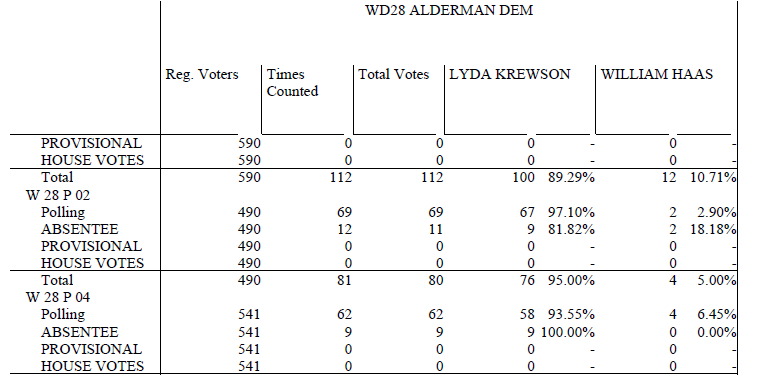
\includegraphics[width=\linewidth]{Figures/CityElection.png} % Replace "image1" with your image file name
            \caption{St. Louis City}
        \end{subfigure}
        
        \vspace{15pt} % Add some vertical space between the subfigures
        
        \begin{subfigure}{0.99\textwidth} % Adjust the width as needed
            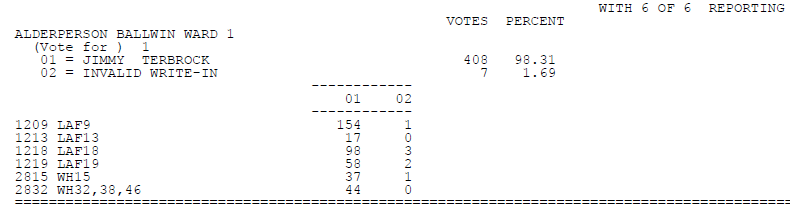
\includegraphics[width=\linewidth]{Figures/CountyElection.png} % Replace "image2" with your image file name
            \caption{St. Louis County}
        \end{subfigure}
        
        \caption[Precinct Level Election Results Example]{Snapshots of official precinct level results from the 2015 General Municipal elections. Both examples cover separate aldermanic races occuring that year.}
        \label{fig:election}
    \end{figure}


    Often, texts include a plethora of information that may not be relevant to our research question. We may only be interested in information when it pertains to specific concepts or is related to particular entities. For example, we may be interested in the kinds of citizens who participate in public town hall meetings and the types of comments they make. A possible text-based source to examine this question would be transcripts of the meetings from the Local View dataset \citep{barariLocalViewDatabasePublic2023}. We would want to extract each commenter's name and comment for each meeting. However, citizens are not the only individuals to participate in these meetings, and we would want to filter out public officials who may be leading the discussion. Citizens may also talk in groups or multiple times throughout a meeting, and we would like to associate each citizen with all the comments they make. Human coders could, albeit tediously, accomplish this task as they could understand both the context as to whether an individual was a citizen and whether each transcribed portion of the meeting belonged to a specific individual. In the case of automated approaches, this task can quickly grow in complexity, as even if automated approaches can identify comments and commenters, researchers would be forced to devise a schema to filter out unwanted participates and to associate comments with individual commenters.\footnote{I should note that recent advances NER and OCR based approaches can successfully associate entities within texts, but they would likely still require some amount of training and fine-tuning to function successfully \citep{kimOCRfreeDocumentUnderstanding2022}} The need for context around information need not even be so complex. It can be as simple as only wanting specific dates or monetary values from texts, both of which might require some level of contextual awareness to identify correctly.

    Transforming text-based sources is not an impossible task, but hand coding can be costly in terms of time and resources, and automated approaches often require significant labor to get up and running and are inflexible to new cases. There is a need for an approach that combines the adaptability of hand coding with efficient automated approaches. I propose that we can employ LLM to meet this need and improve the number and variety of text-based sources we transform into usable datasets.



    \section{What are LLMs and How Can They Help?}
    The term LLM refers to a family of deep learning models built upon a \textit{transformer} framework \citep{vaswaniAttentionAllYou2017}. Hallmarks of these models include immense training sets comprised of a variety of text sources ranging from web content, code, or even classical literature and billions (or, at the time of writing, trillions) of individual parameters, which allow these models to understand the human language on a previously unprecedented level \citep{adiwardanaHumanlikeOpenDomainChatbot2020,brownLanguageModelsAre2020,radfordLanguageModelsAre2019}. While there currently exists a plethora of LLMs, each with its unique size, scope, and intended purpose, in the interest of this paper I will focus primarily on the application of large generative language models such as OpenAI’s GPT-3 \citep{brownLanguageModelsAre2020}, Google’s Lambda \citep{thoppilanLaMDALanguageModels2022} or the open-sourced LLama \citep{touvronLLaMAOpenEfficient2023} and BLOOM \citep{scaoBLOOM176BParameterOpenAccess2023} models. At the most basic level, these larger models are trained to predict words and phrases in response to some initial prompt or context. For example, when presented with the question “What color is the sky?” the model may respond with “Blue” as this is the most probable response to the initial question.\footnote{This is a general overview of how these models function. Models include a variety of other features, such as context windows or temperature. Models can also be trained with additional Reinforcement Learning with Human Feedback (RLHF), which influence a model's ability to respond to specific contexts \citep{ouyangTrainingLanguageModels2022}.}

    Despite the seeming simplicity of this design, these models have shown a remarkable ability to perform emergent capabilities ranging from replicating common natural language processing tasks (e.g., sentiment analysis, classification, and topic modeling) \citep{brownLanguageModelsAre2020,ornsteinHowTrainYour}, to performing information retrieval tasks \citep{zhouFrequencybasedDistortionsContextualized2021}, or even generating synthetic human responses to survey questions \citep{argyleOutOneMany2023}. LLMs perform these emergent tasks by changing the core tasks into a series of next-word prediction tasks. Models are presented with some form of prompt or initial context and then tasked with generating a response in accordance with some set of rules. For example, a researcher interested in obtaining the sentiment of tweets might ask the model whether a tweet is positive, negative, or neutral in tone and then provide the tweet's text. The model would then give the most probable response from that selection of options. To further improve a model's performance, researchers can provide examples of desired responses, commonly referred to as one or few-shot learning examples \citep{lazaridouInternetaugmentedLanguageModels2022}.

    I propose that we can turn the transformation of text-based sources into a next-word prediction task and then have these large-scale models complete them as synthetic coders. By providing these models with our text-based source and a prompt detailing how we want it processed, we can leverage the advanced capabilities of these models to transform texts in an adaptable and efficient fashion. Specifically, I suggest we provide these models with instructions—much akin to instructions for human coders—regarding the type of information we want from texts and then have the model identify, extract, and format said information into quantifiable datasets. These models' ability to understand the contextual features of text allows them to overcome many of the hurdles associated with prior automated approaches and produce near-human-quality coding responses. However, these models should not synthetically code all text-based sources without validation.

    While impressive, LLMs have several limitations that may negatively affect their ability to code text-based sources. First, these models are trained on a large variety of human-generated data and, as such, can express many of the same biases and stereotypes present within these data \citep{gargWordEmbeddingsQuantify2018,caliskanSemanticsDerivedAutomatically2017,benderDangersStochasticParrots2021,zhouFrequencybasedDistortionsContextualized2021}. These reflected biases may be especially concerning for political science research as models may systematically misidentify information pertaining to marginalized groups. For example, a model tasked with identifying government officials with a piece of text may inappropriately identify (or misidentify) individuals along the lines of gender or race. Second, these models can produce noisy results or hallucinate data not initially present within the original text \citep{linTruthfulQAMeasuringHow2022}. In either case, the incorrect data may be difficult to spot and contaminate the final dataset in unseen ways. Given these potential problems with LLMs, researchers must have some way to validate the output of these models \citep{grimmerTextDataPromise2013,knoxTestingCausalTheories2022}. Therefore, in the following section, I propose a human-in-the-loop process in which researchers iteratively design the context for these models and then validate their performance on a subset of their data to identify—and ideally minimize—instances of error and bias.

    \section{The Proposed Pipeline}


    Following many of the principles from recent advances in adaptive machine learning \citep{enamoradoUsingProbabilisticModel2019,wiedemannProportionalClassificationRevisited2019,millerActiveLearningApproaches2020}, the framework relies on leveraging LLMs efficiency to process some text-based sources and then utilizing humans to correct and guide these models to the correct answer \citep{mozerMatchingTextData2019}. While most applications of adaptive machine learning rely on the models to iteratively update based on human input, this process follows an alternative approach. Much like a researcher would update instructions for human coders, the researcher updates parameters and inputs in response to the model's performance. The process consists of hand coding a subset of data and then using that data to improve the prompt and context sent to the LLM iteratively. Once the LLM achieves a researcher's desired level of accuracy, it is used to transform the remaining data. \autoref{fig:workflow} provides an overview of each of the steps within the workflow. Notably, the process overall is agnostic to the exact LLM utilized, but as detailed below, the model's characteristics may substantially affect a researcher's choices throughout the process.

    \begin{figure}[H]
        \centering
        \begin{tikzpicture}
            % Define nodes
        \node[draw,
        rounded rectangle,
        minimum width=2.5cm,
        minimum height=1cm] (block1) {Preprocess Text};
     
     
        \node[draw,
        rectangle,
        below=of block1,
        minimum width=2.5cm,
        minimum height=1cm] (block2) { Subset and hand code training set};
     

        \node[draw,
        rectangle,
        below =of block2,
        minimum width=2.5cm,
        minimum height=1cm] (block3) {Create prompt with instructions};
    
        \node[draw,
        rectangle,
        below =of block3,
        minimum width=2.5cm,
        minimum height=1cm] (block4) {Choose text context};

        
        \node[draw,
        rectangle,
        below =of block4,
        minimum width=2.5cm,
        minimum height=1cm] (block5) {Process training data with LLM};

        \node[draw,
        rectangle,
        below =of block5,
        minimum width=2.5cm,
        minimum height=1cm] (block6) {Evaluate LLM performance};
    
        \node[draw,
        rectangle,
        below=of block6,
        minimum width=2.5cm,
        minimum height=1cm] (block7) {Process unlabeled data};

        \node[draw,
        rectangle,
        right =of block4,
        minimum width=2.5cm,
        minimum height=1cm] (block8) {Repeat until model achieves set error rate};
    

        \draw [arrow] (block1) -- (block2);
        \draw [arrow] (block2) -- (block3);
        \draw [arrow] (block3) -- (block4);
        \draw [arrow] (block4) -- (block5);
        \draw [arrow] (block5) -- (block6);
        \draw [arrow] (block6) -- (block7);
        \draw [arrow] (block6) -| (block8);
        \draw [arrow] (block8) |- (block3);
        

        \end{tikzpicture}
        \caption[Framework for using Large Lanaguage Models to transform text-based sources.]{Framework for using Large Lanaguage Models to transform text-based sources.}
        \label{fig:workflow}
    \end{figure}

    \subsection{Preparing Text-Based Sources}
    The first step of the workflow is to preprocess the text into some machine-readable format. Like most text-as-data approaches, how we preprocess the text can significantly affect our final results \citep{grimmer2022text,wilkersonLargeScaleComputerizedText2017}. However, unlike most preprocessing for NLP, we want to be careful not to remove too much from the texts. We want our text to maintain its rough format and maintain any important contextual features surrounding our desired data. For texts that require some form of OCR, as is the case with many legal and government documents, we need to be aware that the quality of the transformed text may affect their data of interest. Poorly converted data can inhibit even LLM's performance by potentially obfuscating our desired data within the text \citep{vanstrienAssessingImpactOCR2020}. 

    Next, we must divide some of our texts into a training set. This training set aims to validate the LLM's performance, so it should represent a wide variety of texts within our corpus. If we draw on texts from multiple sources, the training set should include examples from each source. Similarly, if we rely on text spanning numerous years, the training set should consist of some texts from each period present within the corpus. For each text within this set, we must manually code the text into our desired data format. This set will be used as the golden standard to compare the performance of the LLM. There is no hard-set rule regarding the size of a training set, although most conventual splits for machine learning rely on splitting at least 20 percent of the sample into a training set. Notably, larger training set sizes will allow researchers to better check the LLM's performance at the cost of additional hand coding.\footnote{Several notable advances have been made in optimizing one's choice in training sets \citep{kaufmanSelectingMoreInformative2024}. Although it is not clear whether they could be applied in this context.} After successfully dividing our corpus, we can begin constructing the prompt for our LLM.

    \subsection{Selecting a Prompt and Context}
    Much like human coders, models require some form of text-based instructions to generate responses. This prompt details the instructions for the model and will be our primary point of iteration and revision throughout the workflow. While the exact wording of our prompt will vary depending on our text and desired data, the prompt should include three key components. First, we should specify the information we wish to extract from the text. We should be as specific as possible in this stage, as more detailed descriptions tend to lead to higher-quality outputs from the model. Second, is the format we want the model to return our data in.\footnote{Given most LLMs are trained on a large body of code, we may opt to have the model return the results in a data format from our preferred coding language (e.g., a data frame within R, or a dictionary within Python).} Beyond making it easier to process the data output from the model, having a consistent output can make it easier for us to detect errors. In addition to these formatting instructions, we should provide instructions on what the model should do when the desired data is absent from a text. By doing so, we can reduce unexpected responses from the model and provide a clear null case during the validation step. Finally, a one or few-shot learning example of the desired output data. For example, again, in the case of obtaining sentiment from a tweet, we would want to include examples of tweets and their respective coding. These training examples can significantly improve an LLM's performance and help the model produce consistent results \citep{brownLanguageModelsAre2020}. If including a full training example is not feasible due to the type of desired data or length of the text, we can include an example output to obtain a similar effect on model performance and consistency.\footnote{I show an example of this practice within both case studies later in this article.}

    Our last choice in the workflow is the context of the text to share with the model. Specifically, how much of the text-based source should be included following the prompt? All LLMs have a maximum sequence window. These windows are primarily a factor of the model's number of parameters and effectively dictate how much text the model can intake and output at a time. Most models have context windows between 2048 and 8000 tokens.\footnote{Tokens are sequences of characters representing meaningful units of text. Usually, tokens consist of one or more words, but different models utilize different tokenizers to preprocess text.} Given these limits, we must be careful regarding how we present our text to the model. For smaller texts, we can freely include the entirety of the text following the prompt. However, for larger texts, we may need to split the text into sections and have the model process each section. If we break our texts, we should consider how the splits may affect our desired information. We may inadvertently split a section of desired information and effectively cut it out of the text we provide the model. Beyond context windows, we may want to give the model specific sections of text to limit the chances of false positives or cut down on the total text sent to the model. For example, if we only care about information present at the beginning of a document, it would be faster and potentially safer only to provide said section to model rather than the entirety of the text. However, if our desired information could occur throughout a text, we would need to give the entirety of the text to the model.

    Before we process our training data, we may need to decide on a few additional model parameters. These parameters vary between models but often include a maximum response length, a starting seed, or model temperature. Of these parameters, a model's temperature is the most likely to affect the model's capacity to process text-based sources. Conceptually, a model's temperature dictates the diversity in its responses. Often, individuals will equate this parameter to a model's practical creativity. In the context of next word prediction, a model may not choose the most probable word in every case and instead choose an alternative, less likely word or phrase. Given this workflow aims to produce consistent results from text-based sources, we will want to use lower model temperatures.

\subsection{Processing, Iterating, and Validating}
    With our prompt, context, and ancillary parameters decided, we can finally ask the LLM to transform our training data. Most LLMs can be sent data directly through an API.\footnote{Popular models often also include an official or popular open-sourced package that facilitates interacting with their APIs in the most popular coding languages (see the ```text2data``` package from \citet{ornsteinHowTrainYour} as an example.)} For each text within our training set, we will send the model our specific prompt and context and then store its response. Since it can be difficult to anticipate whether our early prompts will be effective, we may want to start with a small portion of our training set and slowly incorporate more of our data as we finetune the model.

    After the model processes our training set, we will evaluate its performance using standard accuarcy and calibration metrics . While we will need the model's overall performance to report our uncertainty later, we want to focus on instances in which the model failed to transform text or mislabeled data for the initial iterative process. Were there certain types of text the model failed to process? Does the model include irrelevant data in its response? Did the model show any obvious signs of bias in the data that it correctly or incorrectly identified? Common corrections we may make in response to these questions are increasing the text sent to the model, changing a prompt to be more specific, changing the learning examples, specifying additional cases to exclude from the output, or breaking up transform into separate steps.\footnote{If we are interested in many pieces of information, creating a different prompt for each piece may be more effective.} After correcting our prompt and context, we can repeat our workflow until the model's output is sufficiently similar to our hand-coded data. Like any machine learning approach, LLMs will likely never perfectly correspond to our training data. However, as I highlight in later case studies, obtaining accuracy metrics between 80\% and 95\% is not unreasonable. If we desire to push the model's performance beyond these limits, we may risk effectively "overfitting" to our training set. This "overfitting" can be problematic if our set is not representative of our larger corpus or if we want to transform a new data set.\footnote{To alleviate overfitting concerns, we may wish to hold out a portion of the training set as a validation set for our final model parameters.}  

    Once our model reaches our desired level of accuracy, we can send our unlabeled text to the model. If any errors occur in this process, we may want to adjust our training set to incorporate problematic texts and reiterate through the workflow. After we process all unlabeled texts, we should record our chosen LLM, last prompt, context, and model accuracy and present them clearly within our final results.


    \section{Applications and Validation}

    In the following two applications, I demonstrate how LLMs can efficiently and accurately transform text-based sources into high-quality data. For both applications, I use OpenAI's GPT 3.5-turbo-1106 to identify, extract, and format meaningful information from text-based records across two starkly different areas of political science. I validate the model's performance with a comparison to its predicted performance from the iterative workflow and human-coded data. Examples of each text-based source and how they were processed can be found in Section C.1 of the Appendix.

    \subsection{Extracting Commenters From Local Meeting Minutes}
    Understanding who and how individuals participate in local governmental meetings has become a key area of study for urban politics \citep{einsteinWhoParticipatesLocal2019,einsteinStillMutedLimited2022,yoderDoesPropertyOwnership2020,nuamahCostParticipatingPoor2021,collinsDoesMeetingStyle2021}. Much of this research relies on datasets of political participation constructed directly from publicly available meeting minutes. In many cases, these minutes record the names, comments, and, at times, addresses of those who participate in public meetings. However, extracting this fruitful data takes work. Meeting minutes, while by law include similar information, such as the names of public officials, votes on local policies, and public commenters, they do not follow similar formats.

    The laws mandating meeting minutes frequently lack specificity, and it is up to the local government to determine the style and level of detail in these recorded minutes \citep{oconnorAssemblyRequiredApplication2004}. As a result, meeting minutes can vary substantially in detail and style between any two local governments.\footnote{Section C.1 within the Appendix provides a select sample of minutes from two similar sized cities within the St. Louis region.} Formatting within governments can even change as new governmental clerks are appointed or the government adopts new strategies, formats, or technologies. These limitations make constructing a diverse and longitude dataset of meeting participation an extremely time-intensive task. As a compromise, research within this area often focuses only on a handful of similar local governments \citep[e.g.,][]{yoderDoesPropertyOwnership2020,einsteinWhoParticipatesLocal2019} or infers participation based on national survey responses \citep{nuamahCloseHomePlaceBased2021}. These compromises, however, come at the cost of potentially noisy estimates and limited variation in the types of local governments examined.

    A demand exists within the field to alleviate the burden of processing these minutes, and LLMs could effectively address this need. To demonstrate how LLMs can be applied to this problem, I apply the workflow above to select school board meeting minutes from the St. Louis region. The dataset consists of all the general meeting minutes from 2018 to 2022 for 16 school boards. The data includes 667 separate meetings ranging immensely in style and detail. This sample should provide a wide variety of meeting minutes between local governments and a perfect test of the capabilities of LLMs.

    I start by hand coding each meeting's minutes and extracting the commenters, addresses, and comments for each meeting. In reality, most researchers will only label a small sample of the data, so to mimic that, I randomly select ten meetings from each government to represent my initial training set of 160 meetings. Next, I construct an initial prompt and display the final prompt in  \autoref{fig:meetingprompt}. Given that public comments can occur at any place within a meeting, I feed the model the entirety of the meeting text. For longer meetings, I split the meetings into 3,000 token chunks. I set the model's temperature to 0 and then feed in each meeting with the associated prompt. To evaluate the model, I examine whether the model obtained the full names, addresses, and comments of each commenter within my training set of meetings.\footnote{In the case of the comment's text, I only examined whether the model returned a comment and not necessarily whether the comment's text matched perfectly.} After approximately four iterations of adjusting the prompt, with the primary changes being additional specificity and modifications to the example outputs, the model displayed a precision of 0.934, recall of 0.984, and F1 of 0.957 for the training set. Given these promising estimates, I fed the remaining meeting through the model and evaluated its performance on the entire dataset.

    \begin{figure}[H]
        \centering
        \begin{lstlisting}[language=python,  label={fig:meetingtext}]
        In the following text of recorded public meeting minutes
        can you identify all of the commenters who spoke during 
        the public comment period(s), all of their addresses if 
        available, and all of their complete comments. 
        Return them in a JSON format. Please do not include public
        officials and use NA for any missing information.
        
        Example Output: 
        
         {
          "Name":["Shawn Spencer"],
          "Address":["5005 North Fraser Way"],
          "Comment":["Concerns about recent crime in the community"]
          }
        
        If no one commented please return: 
        
         {
          "Name":["No Commenters"],
          "Address":[""],
          "Comment":[""]
          }
        
        Meeting Text:
        [MEETING MINUTE TEXT]
        
        \end{lstlisting}
        \caption[Prompt to Extract Commenters from Public Meeting Text Using GPT-3]{Prompt to extract commenters from public meeting text using GPT-3}
        \label{fig:meetingprompt}
    \end{figure}

    Overall, the model could accurately extract almost all commenters from the meeting minutes dataset with an average precision score of 0.935. Incredibly, the model exhibited a low false positive rate with an average recall of 0.977. To contextualize these findings, an untrained BERT NER model only achieved a precision of 0.780 and recall of 0.850, requiring extensively more coding and filtering of results.\footnote{More details on the NER application can be found within the Appendix.}  While the LLM successfully parsed most meeting minutes, it failed in a few select cases. The LLM tended to code meetings inaccurately, in which school boards only included the number of total commenters without any form of identifying information. If we would be interested in the count in addition to the commenter's details, we would need to adjust the prompt accordingly or construct a separate one. Another area in which the model struggled was when individuals made detailed and lengthy comments. In these cases, the model would occasionally truncate the comment down. Adjusting the context of the text remedied this problem, but not completely.

    In terms of time to code, the model took approximately 3 hours to fully parse all the meeting minutes at a cost of roughly \$0.01 per meeting. Including the training, the model costs \$8.28 to process the dataset. In comparison, human coding the dataset required an estimated 15 hours to parse the meeting minutes. Beyond being faster and less costly, utilizing an LLM could allow us to parse meetings multiple times for other forms of information, such as the meeting format, the names of public officials, and other critical pieces of information, all only requiring us to hand code a small sample of the entire data.

    
    \subsection{Identifying Interest Groups in Amicus Curiae Briefs}
    Amicus briefs are a valuable tool to estimate interest group's political participation before the Supreme Court. Beyond simple participation, they can reveal underlying political networks \citep{Box-Steffensmeier:2015b}, track  groups' political influence \citep{box-steffensmeierQualityQuantityAmici2013}, and  provide measures of group ideology \citep{abi-hassanIdeologiesOrganizedInterests2023}. To utilize these records, previous researchers hired coders to go brief by brief and extract the names of interest groups and the legal direction of the brief in a time-intensive process. As highlighted previously in this article, the core difficulty with extracting this valuable information from these documents is that organizational names can come in various formats and can vary in their exact placement at the beginning or end of a brief. Identifying the legal direction of a brief is more straightforward as most briefs explicitly state the party they support; however, in a few cases, briefs may report support or opposition of a lower court decision rather than a case's litigants. The combination of varying formats and locations can make correctly identifying either the signers or legal direction difficult, even for human coders. Expediting the processing of these briefs could bring numerous benefits, from easing the maintenance of existing datasets, expanding the coverage of included briefs, or even examining other novel information within the brief's text. LLMs could be applied to these documents to achieve high-quality results at a fraction of the cost and time.

    To demonstrate this application, I utilize the amicus curiae database from \citet{Box-Steffensmeier:2012d}. I focus on all briefs sent to the Court in 2014. This selection narrows the universe of briefs to process but still provides a diverse sample of 190 individual briefs.\footnote{The Court received 351 total briefs in 2014, but only 190 were publicly available and hand-coded at the time of writing.} Subsetting 40 briefs as my training set, I construct the initial prompt and set my initial context as the first and last five pages of each brief. \autoref{fig:briefText} displays the final prompt used to process the text. In each iteration, I evaluate whether the model correctly identified all signers and separately whether it correctly identified the direction of the brief. Given names may vary slightly between the handing coding and the original text of the brief, I allow for some difference between the two sets of names by utilizing a fuzzy string-matching algorithm to detect a match.\footnote{Specifically, I measure the Damerau-Levenshtein distance between the vectors of names and consider a pair a match if their distance is less than five. Given the names were already close, this distance largely accounted for the inclusions/exclusion of words like “the” or “inc.”} After iteratively adjusting the prompt and enlarging the context to the first and last ten pages of each brief, the model identified brief singers with a recall of 0.922 and precision of 0.90 and the legal direction with an accuracy of 0.975.

    \begin{figure}[H]
        \centering
        \begin{lstlisting}[language=python, label={fig:brief-text}]
    In the following amicus curiae brief, which organizations 
    signed the brief and was it for the petitioner, 
    respondent or neither? Please record the organization
    in the form of a Python dictionary. An example 
    of the output is below and then the text to parse. 
    Do not include the law firm who prepared the brief.
             
    Example Outputs: 
    {
      "AMERICA'S ESSENTIAL HOSPITALS" : "Respondent",
      "NATIONAL FEDERATION OF THE BLIND" : "Respondent",
      "TYRELL CORPORATION" : "Respondent"
      }
    
    {
      "EXXON MOBILE" : "Neither",
      "WEYLAND-YUTANI CORPORATION" : "Neither"
     }
    
    Brief Text:
    [BRIEF TEXT]
    \end{lstlisting}
    \caption[Prompt to Extract Signers from Amicus Curiae Briefs Using GPT-3]{Prompt to extract the name of signers from amicus curiae briefs using GPT-3}
    \label{fig:briefText}
    \end{figure}

    When applied to the remaining data, the model displayed a slightly lower average recall of 0.857 and a precision of 0.867.\footnote{Processing the entire dataset cost \$1.18 and took approximately 30 minutes to complete.} While the model did appear to extract the majority of information from briefs correctly, this drop in performance is concerning as, in real applications, it would be unknown to researchers. Upon closer inspection, two primary factors contributed to the performance dip. First, in some cases, the model would incorrectly format responses, leading to all names being considered incorrect. Often, the model would group two or more organizations rather than separate them in the response. Adjusting the prompt to specify this separation or further parsing the model's results would likely solve this issue. Second, the model would sometimes include individuals or agencies in addition to their parent organizations, whereas previous coders only had one or the other. For example, the model may include both the public finance authority for a city and the city itself as signers. Whether this difference is substantively important is unclear but may be addressed by adding further specificity to the prompt. Regarding identifying a brief's legal direction, the model performed similarly to the training set with an accuracy of 0.956. Overall, using an LLM to code briefs seems to be a feasible approach to accelerate the process while maintaining the quality of the final dataset. Nevertheless, the drop in performance between the training and full datasets underscores the potential vulnerability of relying on small training sets to evaluate an LLM's performance.

    
    \section{Discussion}
    Traditionally, the conversion of text-based sources into meaningful datasets has been a laborious and time-consuming task. However, LLMs present a promising solution to this challenge. These models have the potential to combine the efficiency and speed of traditional automated approaches with the flexibility and adaptability of human coders. By iteratively guiding and validating these models, we can create high-quality datasets at a fraction of the cost and time investment. Furthermore, offering details on how we utilized these models, including the prompt, context, and other parameters, provides a unique opportunity to recreate datasets from their original sources. This form of replication, typically avoided due to its high coding costs, can enhance transparency in using text-based sources and facilitate innovation with existing data. Beyond text transformation, LLMs are a promising tool throughout the research process as they assist researchers in effectively handling various data needs, from formatting data to extracting information or even matching across data sources. However, it's essential to acknowledge that despite these promises, my proposed framework and the broader application of LLMs come with their own caveats and challenges.

    Without coding the entirety of the data, it is impossible to guarantee that coding errors and LLMs' potential biases will not permeate into the datasets they help create. It may be fruitful for future work to explore how we could leverage consensus metrics to combine multiple models to minimize the adverse effects of any particular model. Researchers should also recognize that even in the case of the training set for which we have outcomes to compare, it may be challenging to check for all forms of potential bias. For example, in the case of extracting public commenters, researchers may require additional data such as commenter demographics to gauge whether the misclassifies individuals along the lines of gender or race. Such information is often not widely available and can be difficult to match to the original dataset. Overall, the quality of data produced by the model is a product of the diligence and care researchers put into evaluating and validating the model's performance. Researchers should be transparent regarding their implementation of LLMs and aware of potential biases in their final datasets.

    Additionally, while LLMs may alleviate the burden of transforming data, they do not address the initial burden of gathering it in the first place. A researchers’ choice in which sources to include within their dataset can be just as impactful on their study as how they processed their data \citep{gaikwadTransparencyTextBasedSources2023}.  Hopefully by alleviating the pressures of coding each source, LLM can allow researchers to spend more time gathering novel data or better utilize pre-existing collections of data. The latter benefit may be especially promising given recent innovative data collection efforts such as \citep{barariLocalViewDatabasePublic2023}’s collection of meeting transcripts. Each of which holds to potentially to vastly increase our understanding of each of their respective fields. 

    Overall, Large Language Models (LLMs) are a promising tool for future researchers. Like any tool, they should be implemented with transparency and acknowledgment of their potential limitations. If appropriately used, these models offer the potential to drastically increase the accessibility of political science research and expand the coverage and diversity of data used across research domains.

